\minitoc
\begin{refsection}
\newpage
\fbox{\begin{minipage}{\textwidth}
    \textbf{Contexte :}\\
    Le processus Breit-Wheeler multi-photon a été observé en laboratoire au SLAC en 1997, où de l'ordre de $200$ positrons ont été détectés en $20 ~ 000$ tirs, avec un taux de répétition de l'ordre du Hertz. Le processus Breit-Wheeler linéaire n'a quant à lui jamais été directement observé en laboratoire depuis sa prédiction en 1934 (chapitre \ref{chap:1-particules}), même si plusieurs schémas de principe d'expériences ont été proposés depuis 2014. 
    
    \medskip
    \textbf{Résumé du chapitre :}\\
    Dans ce chapitre, les propositions publiées avant fin 2020 sont présentées. Celles-ci font toujours intervenir des photons d'énergie $\gtrsim \si{\MeV}$ produits par les processus Compton inverse linéaire, Compton inverse multi-photon, ou Bremsstrahlung. Ces sources peuvent alors collisionner ensemble, ou avec des photons de plus basse énergies produits par d'autres mécanismes (tableau \ref{fig:3-tableau_propositions}). Dans le cadre de cette thèse, nous nous concentrerons principalement sur les sources de photons produits par Bremsstrahlung, avec un taux de répétition de l'ordre du Hertz (d'autres possibilités seront néanmoins évoquées dans les chapitres suivants). Le schéma de principe d'une cible multi-couches permettant d'atteindre cet objectif est ensuite présenté (figure \ref{fig:3-principe_cibles}), ainsi que la stratégie de détection des positrons élaborée au CELIA conjointement à cette thèse. Ce nouveau concept de détection est basé sur le comptage d'un faible nombre de positrons dans un environnement bruité (figure \ref{fig:3-principe_comptage}). En accord avec cette stratégie de détection, nous nous fixons pour objectif de pouvoir produire de l'ordre de quelques positrons via le processus Breit-Wheeler linéaire par tir laser.
    
    \medskip    
    \textbf{Informations complémentaires :}\\
    Plus d'informations sur les différents schémas de principe d'expériences pour l'observation du processus BWL sont disponibles dans les références indiquées dans le tableau \ref{fig:3-propositions_BWL}. Une revue des problématiques liées à l'utilisation de cibles à taux de répétition important est aussi disponible dans \parencite{prencipe_2017}.
\end{minipage}}
\newpage


\section{Principe de l'expérience}

Dans cette section, nous discuterons de différents schémas de principes expérimentaux proposés pour produire et détecter des positrons créés par collision de photons.
Les résultats obtenus par \cite{burke_1997} lors de l'expérience ayant permis la détection du processus Breit-Wheeler \textbf{multi-photon} seront très rapidement présentés, et serons suivis d'une discussion sur les différentes propositions expérimentales élaborées pour la détection du processus Breit-Wheeler \textbf{linéaire} en laboratoire. Nous verrons alors que celles-ci font appel à des stratégies très variées, et que cette thématique est très actuelle. 

\subsection{Détection du processus Breit-Wheeler multiphoton au SLAC}

Bien que le processus Breit-Wheeler \textbf{linéaire} n'ait jamais été observé pour le moment en laboratoire (voir chapitre \ref{chap:1-particules}), le processus Breit-Wheeler \textbf{multi-photon} à quant à lui \textbf{déjà été détecté} en 1997 au Stanford Linear Accelerator Center par \cite{burke_1997}.

Dans cette expérience, un faisceau de $7 \times 10^9$ électrons de $46.6 ~ \rm GeV$ collisionnait avec un laser \textit{Nd:verre} doublé en fréquence, de longueur d'onde $527 ~ \rm nm$ (photons d'énergie $2.35 ~ \rm eV$), d'énergie totale $650 ~ \rm mJ$, et d'intensité $1.3 \times 10^{18} ~ \rm W/cm^2$ ($a_0 = 0.36$) pour créer des photons $\gamma$ d'énergie allant jusqu'à $29.2 ~ \rm GeV$ via le processus Compton inverse. Les photons énergétiques ainsi produits pouvaient à leur tour collisionner avec le même laser pour produire des paires $e^-e^+$ par le processus Breit-Wheeler multi-photon ($\gamma + n \omega \to e^- e^+$, avec $n \omega$ un nombre $n$ de photons laser), comme représenté sur la figure \ref{fig:3-Burke}a. La conservation de l'énergie implique dans ce cas qu'un minimum de $4$ photons laser ait été nécessaire pour créer une paire $e^-e^+$ (la collision à deux photons nécessitant un photon de haute énergie de plus de $111 ~ \rm GeV$, voir chapitre \ref{chap:1-particules}). Dans cette expérience, les positrons produits avec une énergie cinétique $<20 ~ \rm GeV$ étaient ensuite défléchis par un champ magnétique et détectés par un calorimètre, noté \textit{PCAL} sur la figure \ref{fig:3-Burke}a.

\begin{figure}[hbtp]
	\centering
	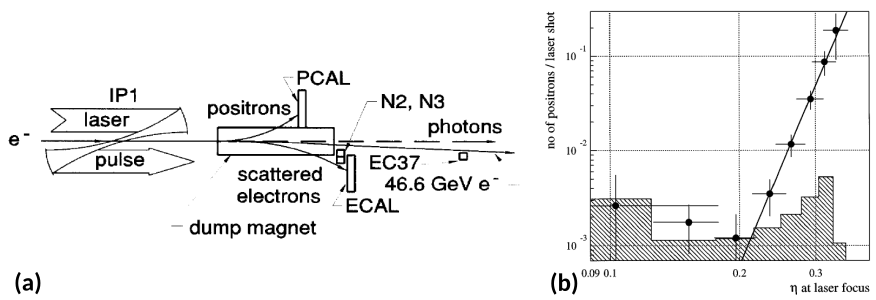
\includegraphics[width=\linewidth]{3-experience/experience_BWM.png}
	\caption{Résumé de l'expérience de \cite{burke_1997} avec (a) le schéma de principe de l'expérience, et (b) le nombre de positron mesurés en fonction du paramètre $a_0$ du laser (noté ici $\eta$). La zone grisée représente ici le bruit de fond, avec un intervalle de 95\% de confiance. Figures tirées de la référence \parencite{burke_1997}.}
	\label{fig:3-Burke}
\end{figure}

Après analyse du calorimètre, $175 \pm 13$ positrons ont été détectés en $21962$ tirs lasers, dont $106 \pm 14$ ne peuvent pas être expliqués par le bruit systématique (zone grisée sur la figure \ref{fig:3-Burke}b). Ces positrons mesurés sont attribués au processus Breit-Wheeler multi-photon, car le bruit de fond et les autres processus connus (notamment le processus Trident multi-photon, voir chapitre \ref{chap:1-particules}) ne permettent pas d'expliquer ce comportement. On peut noter que le \textbf{nombre de positrons détectés par tir est de l'ordre de $10^{-2}$ à $10^{-1}$}, avec un \textbf{taux de répétition de l'ordre du tir par seconde} ($0.5 ~ \rm Hz$).

\subsection{Propositions de schémas expérimentaux pour la détection du processus Breit-Wheeler linéaire}

En 2014, soit presque 20 ans après les résultats obtenus par \parencite{burke_1997}, une expérience qui pourrait permettre de mesurer le processus Breit-Wheeler \textbf{linéaire} en laboratoire (création de paires $e^-e^+$ par la collision de deux photons réels) a été imaginée par O. J. Pike, E. G. Hill et S. J. Rose et F. Mackenroth \parencite{pike_2014}.
Cette proposition, illustrée en figure \ref{fig:3-propositions_BWL}a, ne fait intervenir \textbf{que des lasers} comme sources d'énergie, et implique de faire collisionner un \textbf{faisceau directionnel} de quelques $10^8$ photons autour du $\rm GeV$ avec une \textbf{source X thermique} de température de quelques centaines d'$\rm eV$. La source de haute énergie serait créée en accélérant des électrons par le processus d'\textbf{accélération par sillage}, puis en injectant ce faisceau d'électron dans une feuille d'or pour convertir leur énergie cinétique en photons $\gamma$ par \textbf{rayonnement de freinage} (Bremsstrahlung). La source X serait quant à elle créée par un laser énergétique éclairant un hohlraum (cavité en or) de longueur centimétrique. D'après les premières estimations, la température de la source X semble être d'une très grande importance, et les auteur$\cdot$es estiment qu'en utilisant des lasers actuels de type \textit{Ti:Sa} de quelques $\sim 100 ~ \rm TW$ de puissance pour produire la source de haute énergie, combiné avec un laser de type NIF ou LMJ (énergie de plusieurs centaines de kilo-joules) pour la source X, il serait possible de produire \textbf{jusqu'à $10^2$ à $10^5$ positrons par tir}, selon le nombre et l'énergie des $\gamma$ de haute énergie ainsi que de la température du hohlraum. L'interaction de photons de plusieurs $\rm MeV$ avec la feuille d'or ou avec le hohlraum pourrait néanmoins aussi produire des positrons par le processus Bethe-Heitler ($\gamma Z \to Z e^- e^+$), ce qui compliquerait l'interprétation des mesures.

En 2016, l'utilisation deux sources de photons directionnelles et de plus basse énergie a ensuite été suggérée par X. Ribeyre, E. D’Humières, O. Jansen, S. Jequier, V. T. Tikhonchuk et M. Lobet \parencite{ribeyre_2016}.
Ces auteur$\cdot$es discutent particulièrement de l'opportunité d'utiliser des sources $\gamma$ \textbf{identiques}, à \textbf{haut taux de répétition} (comparé au NIF/LMJ) et d'\textbf{énergie autour du MeV}. Le schéma de principe de cette expérience est illustré en figure \ref{fig:3-propositions_BWL}b. Après avoir discuté de plusieurs possibilités pour la production de telles sources, un modèle théorique et une revue de la littérature leur permis d'établir que les sources \textbf{Bremsstrahlung} et \textbf{Compton inverse multi-photon} seraient les sources les plus crédibles pour ce schéma expérimental. En particulier, des sources Bremsstrahlung \textbf{déjà produites en laboratoire} permettraient selon ce modèle de créer \textbf{de l'ordre de $10^4$ paires BWL par tir}, en considérant la collision de deux sources de photons $\gamma$ produites chacune par un laser de $100 ~ \rm J$ d'énergie. Ce type de sources produit néanmoins de manière inhérente un nombre très important de positrons dans la matière (jusqu'à $10^{10}$, soit de plusieurs ordres de grandeurs supérieur au nombre de paires BWL), pouvant constituer un bruit de mesure pour la détection des positrons BWL. Des sources de photons $\gamma$ produites par \textbf{Compton inverse multi-photon} dans une feuille d'aluminium ou un jet de gaz dense permettraient quant à elles de créer un nombre de paires BWL \textbf{équivalent aux sources Bremsstrahlung} ($\sim 10^4$) avec un \textbf{bruit de positrons plus faible} (entre $10^7$ et $10^9$ d'après les premières estimations), en considérant un laser de 150 J et d'intensité $I_0=10^{23} ~ \rm W/cm^2$. Comme les deux sources de photons sont relativement directionnelles (avec un demi-angle de divergence de $15$ à $30$ degrés typiquement), l'\textbf{angle de collision} moyen entre les sources est aussi un \textbf{paramètre libre} pour l'expérience. Choisir un angle de collision proche de $90$ degrés pourrait alors permettre d'orienter préférentiellement les positrons dans la direction de la bissectrice des deux faisceaux, par un effet cinématique, et ainsi potentiellement faciliter leur détection. Cette possibilité a été étudiée plus en détail pour des collisions de faisceaux de photons mono-énergétiques dans deux articles publiés les années suivantes \parencite{ribeyre_2017, ribeyre_2018}.


En 2017, une étude préliminaire faisant intervenir deux sources \textbf{Compton inverse linéaire}, \textbf{identiques} et \textbf{directionnelles}, produites par le \textbf{couplage de deux lasers avec un collisionneur d'électrons} (ou un collisionneur à électrons-positrons) a été publiée par I. Drebot, L. Serafini, D. Micieli, E. Tassi, E. Milotti et V. Petrillo \parencite{drebot_2017a}.
L'idée d'un collisionneur de photons réels basé sur la diffusion Compton inverse linéaire de lasers dans un collisionneur de leptons n'est néanmoins pas nouvelle, et a été étudiée théoriquement depuis les années 1980 sans jamais être concrètement réalisée. Ce principe est néanmoins toujours discuté actuellement, pour l'étude de collisions de photons de quelques MeV à plusieurs centaines de GeV \parencite{chou_2018, takahashi_2019}. Ce type de schéma expérimental, illustré en figure \ref{fig:3-propositions_BWL}c, permettrait alors non seulement d'étudier le processus Breit-Wheeler linéaire mais aussi la \textbf{diffusion photon-photon}, dont la section efficace est bien plus faible mais est maximisée pour une énergie du centre de masse autour du MeV \parencite{drebot_2017a}. Dans leur proposition, ces auteur$\cdot$es considèrent deux faisceaux d'électrons de $260 ~ \rm MeV$ et $250 ~ \rm pC$ couplés avec deux lasers d'énergie $2 ~ \rm J$, soit des caractéristiques proches de la source de photons $\gamma$ développée pour le projet ELI-NP \parencite{tanaka_2020}. Des \textbf{simulations numériques} prenant en compte les différents processus en présence (processus de collisions photon-photon, mais aussi électron-photon et électron-électron) permettent alors d'estimer le \textbf{nombre d'évènements par tir} comme étant \textbf{de l'ordre de $10^{-4}$}, soit de l'ordre de \textbf{plusieurs dizaines de paires électron-positron détectées par heure} en considérant un taux de répétition de $100 ~ \rm Hz$. Selon ces auteur$\cdot$es, ce type de schéma expérimental pourrait permettre d'étudier le processus Breit-Wheeler linéaire en profondeur (notamment ses effets de polarisation), et représente un défi technique qui leur semble néanmoins raisonnable. D'autres propositions existent pour la détection en laboratoire du processus de diffusion photon-photon réel dans la région du $\rm MeV$, et celles-ci pourraient aussi permettre l'observation du processus Breit-Wheeler linéaire (qui a une section efficace beaucoup plus importante), mais dans la mesure ou cet objectif n'est pas explicitement indiqué, ces propositions ne sont pas détaillées ici (voir les références \parencite{homma_2016, takahashi_2018, takahashi_2019}).


En 2019, la production de paires par collision de \textbf{faisceaux de photons directionnels et identiques} produits \textbf{par laser} via le processus \textbf{Compton inverse multi-photon} fut aussi étudiée par J. Q. Yu,  R. H. Hu,  Z. Gong,  W. J. Ma, C. E. Chen, H. Y. Lu , T. Takahashi, Y. S. Huang et X. Q. Yan \parencite{yu_2019}.
Ces sources de photons énergétiques seraient produites par la propagation de lasers de $10 ~ \rm PW$, du type de ceux de l'installation ELI-NP \parencite{tanaka_2020}, se propageant à l'intérieur de tubes micrométriques vides situés à l'intérieur d'une feuille d'or de quelques centaines de micromètres d'épaisseur. Ce type de source, ayant été préalablement étudiées par l'intermédiaire de simulations PIC 2D \parencite{yu_2019}, seraient à la fois \textbf{très directionnelles} (divergence $<3$ degrés) et \textbf{très intenses} (nombre de photons d'énergie $>10 ~ \rm keV$ de l'ordre de $10^{14}$). Leur collision, illustré en figure \ref{fig:3-propositions_BWL}d, permettrait alors de produire \textbf{jusqu'à $10^8$ paires par tir}, en considérant une distance de collision de $70 ~ \rm \mu m$ et un angle de collision de $170$ degrés entre les deux sources. Le grand nombre de paires BWL produites permettrait alors, selon ces auteur$\cdot$es, de détecter ces positrons en un seul tir avec un rapport signal sur bruit suffisant, et ce en considérant une distance de collision jusqu'à presque $2 ~ \rm mm$, grâce à la faible divergence de ces sources. De plus, le bruit produit par les processus concurrents (Bethe-Heitler, Triplet, ...) serait assez limité dans le tube vide et le nombre de positrons de bruit n’excéderait pas quelques $10^7$. Ces deux derniers aspects ont néanmoins été critiqués et commentés par \cite{wang_2020a} qui \textbf{mettent en doute l'hypothèse des ions immobiles} utilisée dans ces simulations PIC 2D. Ceux-ci montrent qu'en considérant des ions mobiles, la divergence des sources augmente fortement (de l'ordre de $22$ degrés), et le \textbf{nombre de paires BWL produites diminue} d'un facteur $10$ pour une distance de collision de $200 ~ \rm \mu m$. Le \textbf{bruit de positrons} produits par d'autres processus tendrait aussi à \textbf{augmenter}, de part l'interaction de particules énergétiques avec des ions ayant migré dans le tube initialement vide.


Un schéma expérimental très similaire fut aussi étudié par O. Jansen, T. Wang, T. J. Stark, T. Toncian, A. V. Arefiev,  Z. Gong, et D. Stutman dans deux articles distincts, en collaboration avec X. Ribeyre et E. d'Humières précédemment évoqués \parencite{jansen_2018a, wang_2020}. Dans ces références, la collision de deux sources identiques produites par le processus \textbf{Compton inverse multi-photon} est considérée pour des \textbf{lasers plusieurs PW} se propageant dans une \textbf{cible structurée}, composée d'un canal de densité de l'ordre de $10 ~ \rm n_c$ (avec $\rm n_c$ la densité critique) inséré dans une matrice de densité solide (de l'ordre de $100 ~ \rm n_c$ dans les simulations). Le principe de ce type de sources, initialement étudié par \cite{stark_2016}, est illustré en figure \ref{fig:3-propositions_BWL}e, et le schéma de la collision est similaire à la figure \ref{fig:3-propositions_BWL}b. Avec ce type de cibles, et par le biais de simulations 2D \parencite{jansen_2018a} ou 3D \parencite{wang_2020}, ces auteur$\cdot$es estiment qu'ils serait possible de produire \textbf{de l'ordre de $10^4$ paires par tir} à une distance de collision de $250 ~ \rm \mu m$, avec un angle de collision de $90$ degrés. Des estimations ont aussi été menées en considérant un schéma similaire à celui proposé par \cite{pike_2014} et illustré en figure \ref{fig:3-propositions_BWL}a, où la source de photons Bremsstrahlung est remplacée par la source Compton inverse multi-photon précédemment évoquée. Le nombre maximal de paires produites par ce type de schéma serait alors de l'ordre de $10^{5}$ par tir pour un hohlraum centimétrique de température $400 ~ \rm eV$, de l'ordre de $800$ pour une température de 200 eV et seulement 2 paires pour une température de 100 eV. Les auteur$\cdot$es Y. He, T. G. Blackburn en collaboration avec T. Toncian et A. V. Arefiev ont aussi proposé d'utiliser ce type de cible pour effectuer la collision de photons \textbf{à l'intérieur du canal} sous dense, en tirant simultanément avec deux lasers de quelques $10^{22} ~ \si{\W\per\cm^2}$ d'intensité de chaque côté du canal \parencite{he_2020}. Il est alors montré que le nombre de paires produites par le processus BWL peut atteindre \textbf{plusieurs $10^8$ paires par tir} et est très supérieur au nombre de paires produites par le processus Breit-Wheeler multi-photon. Les paires produites seraient alors\textbf{ collimatées dans l'axe de propagation laser}, et pourraient être accélérées à des énergies cinétiques supérieures à $200 ~ \si{\MeV}$. 

Enfin, une dernière proposition en date de fin 2020 fut une étude menée par A. Golub, S. Villalba-Chavez, H. Ruhl et C. Müller \parencite{golub_2020}. Ces auteur$\cdot$es y discutent de la possibilité de faire collisionner un f\textbf{aisceaux de photons de l'ordre du GeV}, produits par \textbf{Bremsstrahlung} via des \textbf{électrons accélérés par sillage}, avec un \textbf{laser à rayons X} (XFEL, pour \textit{X-ray Free Electron Laser}). Le schéma de principe de cette expérience est illustrée en figure \ref{fig:3-propositions_BWL}f. Un modèle analytique leur permet d'estimer l'énergie optimale de la source d'électrons, ainsi que l'épaisseur optimale du convertisseur permettant de maximiser la production de paires BWL. Sous ces conditions optimales, et avec un laser à rayons X d'énergies $0.3 ~ \rm keV$, il est estimé qu'il serait possible de produire \textbf{jusqu'à $350$ paires par tir}, en faisant collisionner les deux faisceaux à une distance de $40 ~ \rm cm$. Les électrons et positrons émis par BWL seraient alors préférentiellement orientés dans la direction du faisceau de photons Bremsstrahlung, avec une énergie autour de $600 ~ \rm MeV$. La propagation de particules énergétiques dans la matière constitue néanmoins ici aussi une source de bruit de positrons importante. Cette proposition serait en principe réalisable sur les installations du projet HiBEF \parencite{hibef}.

\begin{figure}[hbtp]
	\centering
	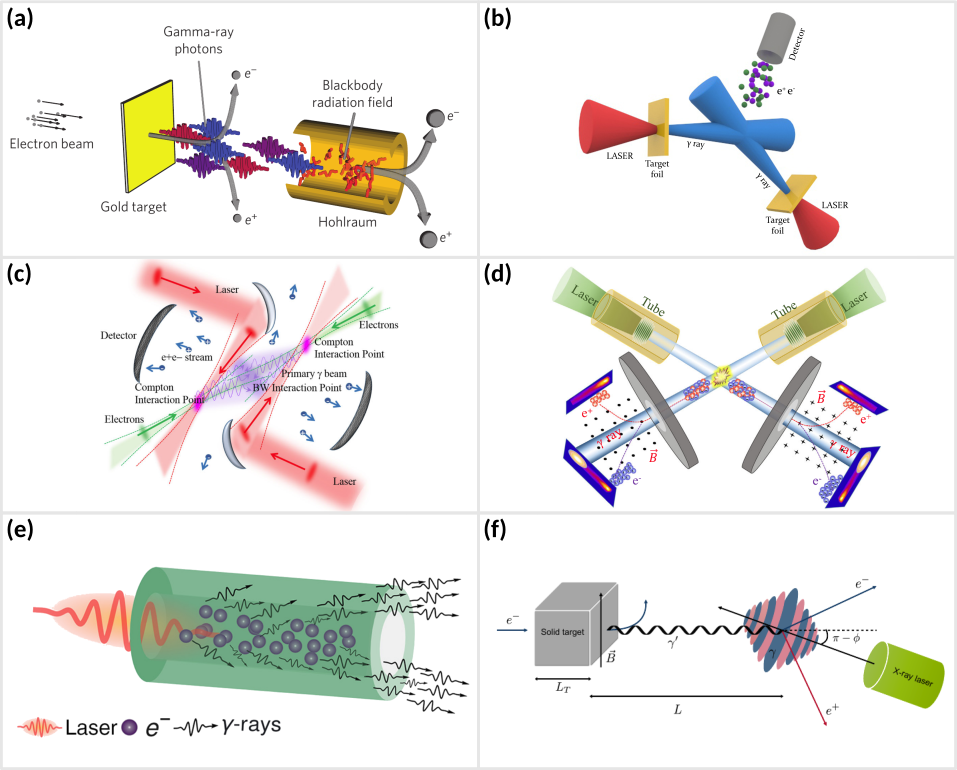
\includegraphics[width=\linewidth]{3-experience/experiences_BWL.png}
	\caption{Illustrations des propositions expérimentales pour l'observation de la création de paires par collision de photons réels, avec (a) la proposition de \cite{pike_2014} faisant intervenir une source Bremsstrahlung avec une source X thermique, (b) la proposition de \cite{ribeyre_2016} faisant intervenir deux sources Bremsstrahlung ou Compton inverse multi-photon, (c) la proposition de \cite{drebot_2017} faisant intervenir deux sources Compton inverse linéaire, (d) la proposition de \cite{yu_2019} faisant intervenir deux sources Compton inverse multi-photon, (e) une illustration du principe des sources initialement proposées par \cite{stark_2016} et appliquées à la production de paires BWL dans \cite{jansen_2018a} et \cite{wang_2020}, et (f) la proposition de \cite{golub_2020} faisant intervenir une source Bremsstrahlung et un laser à rayons X (XFEL). Les figures proviennent respectivement des références \parencite{pike_2014}, \parencite{ribeyre_2016}, \parencite{drebot_2017a}, \parencite{yu_2019}, \parencite{wang_2020} et \parencite{golub_2020}.}
	\label{fig:3-propositions_BWL}
\end{figure}

\subsection{Résumé des propositions}

Comme nous pouvons le constater sur la figure \ref{fig:3-propositions_BWL}, les approches actuellement envisagées pour l'observation du processus BWL peuvent être assez diverses. Certaines considèrent la collision d'un faisceau directionnel de photons d'énergies dans la gamme du $\rm GeV$ avec un rayonnement relativement peu directionnel et peu énergétique dans la gamme de la centaine d'$\rm eV$, telles que les propositions de \cite{pike_2014} et l'étude de \cite{wang_2020}. D'autres proposent au contraire de faire collisionner deux faisceaux de photons identiques, directionnels, et d'énergies autour du $\rm MeV$, telles que les propositions de \cite{ribeyre_2016}, \cite{drebot_2017}, \cite{yu_2019},  \cite{wang_2020} et \cite{he_2020}. Une autre possibilité est l'utilisation de deux faisceaux directionnels mais d'énergies très différentes, l'un dans la gamme du $\rm GeV$ et l'autre dans la gamme du $\rm keV$, telle que la proposition de \cite{golub_2020}. Ces différentes approches sont résumées en figure \ref{fig:3-tableau_propositions}. Nous rappelons que le seuil de création de paires est donné par la condition $E_{CM} = \sqrt{2 E_1 E_2 (1-\cos{\psi_{12}})}>2 m_e c^2$, où $E_1$, $E_2$ est l'énergie du photon 1, 2 respectivement, et $\psi_{12}$ est l'angle de collision entre les photons.

\begin{figure}[t]
	\centering
	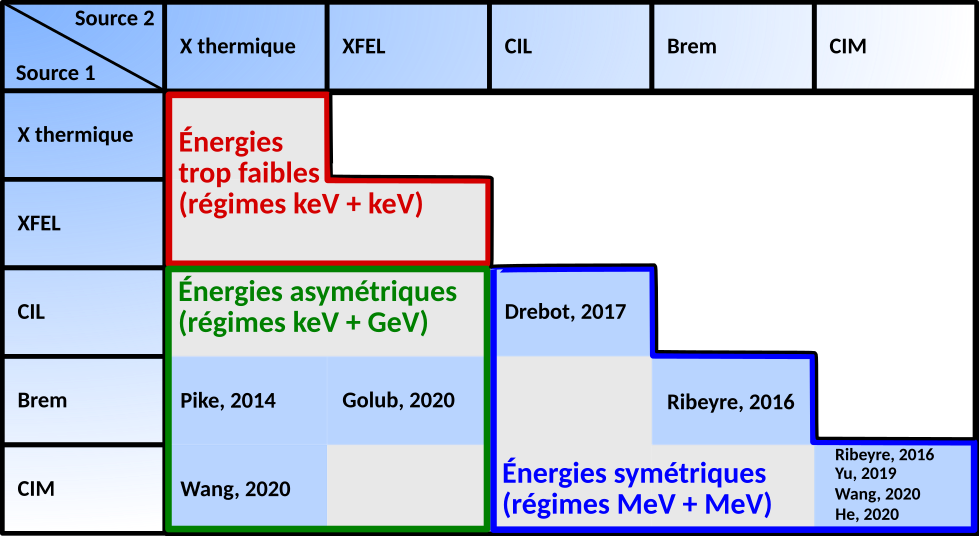
\includegraphics[width=\linewidth]{3-experience/tableau_experiences.png}
	\caption{Résumé des propositions expérimentales pour sur la création de paires par BWL, en début 2021. XFEL signifie X-ray free electron laser, CIL signifie Compton inverse linéaire, Brem signifie Bremsstrahlung, et CIM signifie Compton inverse multi-photon. La collision de deux sources dans le régime keV (de quelques 100 eV à quelques 10 keV) ne permet pas de produire des paires car l'énergie de la collision est trop faible. Ces sources peuvent néanmoins produire des paires BWL en collisionnant avec des photons dans la gamme du GeV (entre 100 MeV et quelques GeV). La collision de deux sources d'énergies dans le régime du MeV (entre 100 keV et 100 MeV) est aussi possible. Le coin supérieur droit du tableau est symétrique par rapport à la diagonale.}
	\label{fig:3-tableau_propositions}
\end{figure}

Dans ces différentes stratégies, le nombre de paires produites par tir et le taux de répétition sont aussi très variables, allant d'un nombre de paires de $10^{-4}$ par tir avec un taux de répétition de $100 ~ \rm Hz$ pour \cite{drebot_2017} à un nombre de paires de $10^5$ par tir mais avec un nombre de tirs très faible (limité par la cadence des grosses installations NIF/LMJ) pour \cite{pike_2014}. Le nombre de positrons produits par d'autres processus dans la zone d'interaction est aussi très différent, pouvant être inférieur à la production de paires par BWL pour \cite{drebot_2017} à très largement supérieur au nombre de paires produites par BWL, pour les propositions faisant intervenir des sources Bremsstrahlung telles que les propositions de \cite{pike_2014}, \cite{ribeyre_2016}, ou \cite{golub_2020}. Les sources de photons produites par Compton inverse multi-photon ont aussi pour le moment seulement été étudiées via des simulations numériques, alors que des sources Bremsstrahlung sont produites par laser en laboratoire depuis les années 1990 (voir chapitre \ref{chap:2-laser}). Enfin, certaines propositions nécessitent l'adaptation d'installations existantes telle que la proposition de \cite{drebot_2017}, et certaines seront possibles sur des lasers actuellement en construction, comme les propositions de sources Compton inverse multi-photon de \cite{ribeyre_2016}, \cite{yu_2019}, \cite{wang_2020}, \cite{he_2020} alors que d'autres pourraient a priori être effectuées sur des installations déjà disponibles, comme les sources Bremsstrahlung de \cite{pike_2014}, \cite{ribeyre_2016} ou \cite{golub_2020}. 

Dans le cadre de cette thèse, nous nous concentrerons principalement sur l'étude de \textbf{sources de photons identiques, directionnelles, dans la gamme du MeV}, telles que proposées dans \cite{ribeyre_2016}. Pour des sources crées par les processus Bremsstrahlung ou Compton inverse multi-photon, le \textbf{nombre de positrons produits par BWL} sera \textbf{faible devant le bruit de positrons créés par d'autres processus}. 
D'autres particules énergétiques (électrons, photons, ...) ou des ondes électromagnétiques produites lors de l'interaction laser-plasma pourraient aussi interagir avec et perturber l'appareil de mesure. Pour pouvoir attribuer un signal mesuré à la détection du processus BWL, il sera donc nécessaire de \textbf{filtrer} et de \textbf{bien caractériser} le \textbf{bruit de mesure}.

\section{Cadre de cette thèse}

Dans cette section, nous évoquerons rapidement certaines possibilités de production et la détection de positrons créés par le processus BWL, en considérant des \textbf{lasers de caractéristiques déjà disponibles}.

Nous verrons dans un premier temps que les sources Bremsstrahlung semblent être des candidates crédibles pour la production de photons $\gamma$ avec un taux de répétition de l'ordre du $\rm Hz$. Nous discuterons ensuite d'un schéma de principe de cibles qui pourrait être utilisé pour produire de telles sources de photons. Les développements théoriques et numériques présentés dans la suite de ce manuscrit sont néanmoins adaptés ou adaptables à d'autres processus de production de photons.

Nous discuterons enfin de la stratégie développée conjointement à cette thèse, principalement par J.-L. Dubois et D. Khaghani, pour la détection des positrons produits par le processus BWL. Cette stratégie de détection nous permettra de nous fixer un \textbf{objectif réaliste de production de paire} via le processus BWL, qui sera de l'ordre de \textbf{quelques paires BWL par tir}.

\subsection{Stratégies pour la production de photons gamma}

%chap 2 = 4 types de setup (résumé avantages et inconvénients). Ici : Brem car le + simple dans un premier temps avec des lasers d'énergies modérées (gamme du Joule) (+ haut taux de rep ?). On peux avoir plusieurs modes d'accélération d'électrons (cibles sous-critique, quasi-critique et sur-critique). Ici : on choisit des cibles solides car charge du faisceau d'électron plus importante, et des lasers présentant deux faisceaux courte focale sont d'ores et déjà disponibles (+ autres justif ? cible en un seul bloc ?). Malgré leur plus faible charge, l'utilisation de cibles gazeuses pourraient néanmoins s'avérer pertinentes, en particulier grâce à leur plus faibles divergences ainsi que la possibilité de les utiliser à haut taux de répétition. Nous pouvons combiner quasi-critique + sur-critique (ref exemple et appel figure). De plus, nous nous restreindrons à l'étude de l'incidence normale afin de limiter le nombre de paramètres à faire varier dans l'étude que nous mènerons au chapitre \ref{chap:6-opti_numerique}. Néanmoins, l'étude de l'angle d'incidence pourrait aussi s'avérer intéressante pour cette application (ref Fabien). Ce schéma est un schéma parmi d'autres, et nécessiterait d'être complété par des études ultérieures. Les réflexions théoriques menées au chapitre \ref{chap:5-opti_theorique} considèrent néanmoins aussi des sources produites par CIL et CIM, et la chaine de simu présentée au chapitre \ref{chap:4-methodes_simu} est adaptée à l'étude d'autres situations. D'autres études ont été menées dans les références du tableau \ref{fig:3-tableau_propositions}.

Nous avons vu au chapitre \ref{chap:2-laser} que les installations laser actuelles ou en cours de construction ont des gammes d'énergies, de durée d'impulsion et de taux de répétition diverses. Qui plus est, nous avons montré que plusieurs schéma expérimentaux permettraient de produire des photons d'énergie $\gtrsim \si{\MeV}$ par laser (via les processus Compton inverse multi-photon ou linéaire dans la collision frontale d'un faisceau d'électron d'énergie $\gtrsim \si{\MeV}$ avec un laser plus ou moins intense, via le processus Compton inverse multi-photon lors de la propagation d'un laser d'intensité $\gtrsim 10^{22} ~ \si{\W \per \cm^2}$ dans un plasma sous-critique ou quasi-critique, ou via le processus Bremsstrahlung par injection d'un faisceau d'électrons produit par laser dans un matériau de numéro atomique élevé). Ainsi, de multiples stratégies de production de photons $\gamma$ et de détection de positrons BWL sont envisageables pour cette expérience, tel que cela est illustré par la diversité des propositions résumées dans le tableau \ref{fig:3-tableau_propositions}. 

Les \textbf{lasers actuels} ou en construction avec un \textbf{taux de répétition de l'ordre du Hz} sont généralement limités à des \textbf{énergies de quelques joules à quelques dizaines de joules par impulsion}, et une \textbf{puissance crête inférieure ou de l'ordre du petawatt} (voir chapitre \ref{chap:2-laser}). Pour un laser de durée $30 ~ \rm fs$ (largeur à mi-hauteur) focalisé sur une tache focale de $5 ~ \rm \mu m$ (largeur à mi-hauteur), l'intensité crête de l'impulsion est de l'ordre de $10^{19} ~ \rm W/cm^2$ si on considère une énergie totale de $0.1 ~ \rm J$, de l'ordre de $10^{20} ~ \rm W/cm^2$ pour une énergie totale de $1 ~ \rm J$, ou encore de l'ordre de $10^{21} ~ \rm W/cm^2$ pour une énergie totale de $10 ~ \rm J$. Pour ce type de laser interagissant avec une cible solide ou gazeuse, la production de rayonnement dans la gamme du $\rm MeV$ via le processus \textbf{Compton inverse multi-photon} est généralement \textbf{négligeable} \parencite{ji_2014}, en particulier pour les intensités $\lesssim 10^{20} ~ \rm W/cm^2$. Comme nous avons pu le voir au chapitre \ref{chap:2-laser}, ces gammes d'intensités permettent néanmoins d'accélérer un nombre important d'électrons jusqu'à des énergies de plusieurs $\rm MeV$. En injectant ces électrons dans un matériau solide de numéro atomique suffisamment élevé, ils peuvent alors transférer une partie de leur énergie cinétique dans la \textbf{production de photons d'énergies autour du $\rm MeV$} par le processus \textbf{Bremsstrahlung}. En considérant deux sources de photons produites de cette manière, avec une efficacité d'absorption énergétique du laser dans les photons $\gamma$ de l'ordre de $1 \%$, un demi-angle de divergence de l'ordre de $15$ degrés (valeurs typiques considérées dans \parencite{ribeyre_2016}), et en supposant une distance de chaque source au point de collision de $500 ~ \rm \mu m$, le modèle décrit dans \cite{ribeyre_2016} permet de donner une estimation du nombre de paires produites comme étant \textbf{de l'ordre de $10^{-2}$ paires par tir} pour deux \textbf{lasers d'énergie $0.1 ~ \rm J$}, \textbf{$1$ paire par tir} pour deux \textbf{lasers d'énergie $1 ~ \rm J$}, ou \textbf{$10^2$ paires par tir} pour deux \textbf{lasers d'énergie $10 ~ \rm J$}. \textbf{Le processus Breit-Wheeler linéaire pourrait alors, au moins en principe, être observé en laboratoire sur ce type d'installations à l'aide de deux sources de photons produites via le processus Bremsstrahlung}. La stratégie de détection associée à ce type d'expériences nécessiterait de pouvoir mesurer un \textbf{faible nombre de positrons BWL par tirs} (quelques centaines de positrons par tir tout au plus) dans un \textbf{environnement très bruité} (positrons produits par d'autres processus, particules énergétiques diffusant dans la chambre expérimentale, ondes électromagnétiques produites par l'interaction laser-plasma, …), avec un \textbf{taux de répétition de l'ordre du Hz}.

Pour les études préliminaires menées dans le cadre de cette thèse, nous nous concentrerons donc majoritairement sur l'étude de sources de photons produits par \textbf{Bremsstrahlung}, qui sont bien connues (depuis les années 1990 dans l'interaction laser-solide \parencite{kmetec_1992} et depuis les années 2000 pour un faisceau d'électrons produit dans un jet de gaz \parencite{edwards_2002}) et pourraient notamment être produites sur des installations lasers actuelles, avec un \textbf{taux de répétition de l'ordre du Hz} (un taux de répétition de 500 Hz a déjà été démontré pour des sources produites par interaction laser-solide \parencite{zulick_2013}). Les réflexions théoriques qui seront menées au chapitre \ref{chap:5-opti_theorique} incluent néanmoins également les sources Compton inverse linéaire et Compton inverse multi-photon, et les outils numériques présentés au chapitre \ref{chap:4-methodes_simu} sont en partie adaptés ou pourraient être réadaptés à l'étude de sources Compton inverse multi-photon. Un schéma expérimental permettant de produire des photons $\gamma$ multi-$\rm MeV$ à haut taux de répétition via le processus Compton inverse multi-photon pour des intensités de quelques $10^{21} ~ \rm W/cm^2$ sera aussi rapidement étudié au chapitre \ref{chap:6-opti_numerique}, et des études de collision de photons créés par propagation d'un laser multi-PW dans un canal sous-critique sont disponibles notamment dans les références \parencite{jansen_2018a, wang_2020}.

Pour pouvoir produire ces sources de photons $\gamma$ via le processus Bremsstrahlung, il est tout d'abord nécessaire de produire une source d'électrons suffisamment énergétiques avec un taux de répétition de l'ordre du Hz. 
Nous proposons ici d'étudier particulièrement les \textbf{cibles solides}. En effet, nous avons vu au chapitre \ref{chap:2-laser} que l'énergie cinétique des électrons peut atteindre quelques MeV dans l'interaction laser-solide dès lors que l'intensité dépasse quelques $10^{18} ~ \rm W/cm^2$, et que la charge totale du faisceau d'électrons accéléré y est en général plus importante que pour les sources d'électrons produites par accélération par sillage dans un jet de gaz sous-critique. Ce choix pourrait néanmoins être critiqué, et des études complémentaires reposant sur d'autres modes d'accélération pourraient s'avérer utiles.
Dans l'étude numérique qui sera menée au chapitre \ref{chap:6-opti_numerique}, nous considérerons des sources d'électrons composées de cibles bi-couches, où une couche de matériau quasi-critique nommée ici \textit{absorbant} sera fixée sur une couche sur-critique nommée \textit{substrat}. Comme nous le verrons au chapitre \ref{chap:6-opti_numerique}, l'utilisation d'un absorbant quasi-critique permet en effet de grandement augmenter l'absorption du laser dans les électrons accélérés. La production expérimentale de matériau de densité quasi-critique est aujourd'hui un domaine de recherche actif \parencite{prencipe_2017, passoni_2020, carrier-vallieres_2017}.
Ce substrat sera accolé à une couche de matériau solide et de numéro atomique élevé, qui permettra de transférer une partie de l'énergie cinétique des électrons en photons énergétiques, et qui sera nommé \textit{convertisseur}. Les électrons produits dans l'absorbant et à l'interface avec le substrat seront donc directement injectés dans ce convertisseur.
Le schéma de principe du type de cibles considérées est illustré en figure \ref{fig:3-principe_cibles}.

\begin{figure}[t]
	\centering
	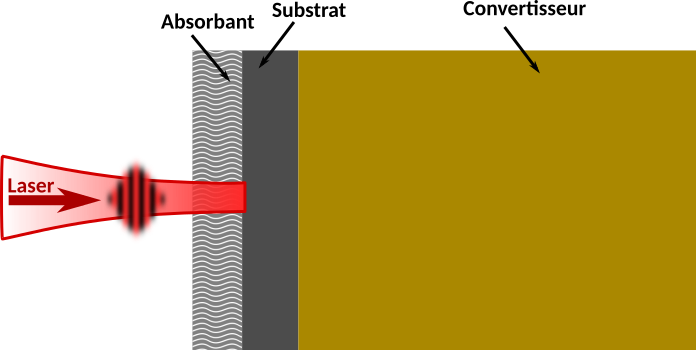
\includegraphics[width=0.7\linewidth]{3-experience/principe_cible.png}
	\caption{Principe des cibles considérées pour la production de photons $\gamma$ par Bremsstrahlung à taux de répétition élevé.}
	\label{fig:3-principe_cibles}
\end{figure}

Il serait aussi éventuellement possible d'ajouter une couche de matériau de haute densité et de numéro atomique faible en face arrière du convertisseur, de façon à diffuser les électrons et positrons produits dans la matière, tout en limitant l'absorption des photons. Cette possibilité a déjà été réalisée expérimentalement \parencite{glinec_2005}, et sera rapidement évoquée au chapitre \ref{chap:6-opti_numerique} sans être étudiée en détail.

Dans le cadre de ces études préliminaires, nous considérerons aussi que le laser interagit en incidence normale avec la cible. Ce choix pragmatique nous permettra simplement de limiter le nombre de paramètres libres à étudier dans l'étude menée au chapitre \ref{chap:6-opti_numerique}. L'étude de la variation de l'angle d'incidence du laser sur la cible pourrait néanmoins s'avérer intéressante pour cette application, car permettant de tirer profit d'autres modes d'accélération d'électrons (voir notamment la référence \parencite{chopineau_2019}). Nous ne rentrerons pas d'avantage dans le détail de ce que la stratégie de taux de répétition du Hz implique d'un point de vue expérimental, ni en terme de stabilité du laser, de production de cibles sur de larges surfaces ou d'alignement de la cible avec le laser par exemple. Ces deux derniers aspects sont notamment discutés dans la thèse de \cite{carrier-vallieres_2017}.

\subsection{Stratégies pour la détection des positrons}

Cette section est dédiée à la présentation rapide de la stratégie de détection des positrons qui a été élaborée conjointement à cette thèse, principalement par J.-L. Dubois et D. Khaghani, respectivement chercheur et post-doctorant au CELIA. Bien que ces aspects n'aient pas été l'objet d'étude de cette thèse, ceux-ci sont néanmoins fortement connectés aux différentes stratégies de production de paires et de gestion du bruit précédemment évoquées.

Comme nous venons de le voir, le défi principal de la détection du processus BWL avec notre schéma expérimental consiste à \textbf{détecter un faible nombre de positrons dans un environnement très bruité}. Il a alors été choisi de réaliser une \textbf{chaîne de comptage} à l'aide d'une \textbf{galette de micro-canaux} (\textit{MCP-PMT}), qui permet d'amplifier fortement le signal reçu (gain de l'ordre de 200 000) et donc de \textbf{détecter les positrons un par un}. 

En plus de cette amplification, un des avantages de ce type de détecteur concerne sa \textbf{réponse temporelle}, annoncée comme étant \textbf{inférieure à 50 picosecondes}. Ainsi, pour des particules se déplaçant à la vitesse de la lumière, la \textbf{zone pouvant contribuer au bruit de mesure} dans cet intervalle temporel est \textbf{limitée à une distance de 1.5 cm autour du détecteur}. En utilisant une photo-diode pour déterminer le temps d'arrivée d'un des lasers sur une des cibles, il sera alors possible de \textbf{filtrer temporellement} le signal de positrons BWL (mesuré juste après l'arrivée du laser) d'une partie du bruit de mesure causé par des \textbf{diffusions de particules} dans l'environnement proche du détecteur, qui peuvent avoir lieu aux temps longs. Le signal reçu depuis cette galette de micro-canaux est aussi proportionnel à l'énergie de la particule incidente.

Une \textbf{lentille magnétique} et un \textbf{blindage approprié} pourront quant à eux permettre de \textbf{limiter le bruit direct de particules} émises par l'interaction laser-cible, telle que les électrons, positrons et photons énergétiques, ainsi que l'effet des impulsions électromagnétiques produites lors de l'interaction laser-plasma \parencite{poye_2015}. En effet, les \textbf{positrons BWL} sont créés à l'\textbf{intersection des faisceaux de photons} et, pour la collision de deux photons d'énergies autour du $\rm MeV$, leur \textbf{direction de propagation} tend à être orientée \textbf{selon la bissectrice de la direction des photons incidents} \parencite{ribeyre_2017}. Au contraire, on s'attend à ce que les \textbf{particules de bruit} produites \textbf{dans la cible} se propagent préférentiellement \textbf{selon la direction de propagation des lasers}. Un blindage approprié pourrait donc permettre de \textbf{filtrer spatialement} ces différents types de particules, par simple effet géométrique, et de sélectionner principalement les positrons produits par le processus BWL. La \textbf{lentille magnétique} permet de plus de \textbf{focaliser les positrons} sur le détecteur tout en \textbf{dé-focalisant les électrons}. Un choix judicieux de la géométrie de la lentille et d'intensité du courant parcourant son bobinage permet aussi de \textbf{sélectionner une gamme d'énergie} donnée pour les positrons.

Le principe de cette chaîne de comptage est illustré en figure \ref{fig:3-principe_comptage} (figure reproduite ici avec l'accord de J.-L. Dubois).

\begin{figure}[t]
	\centering
	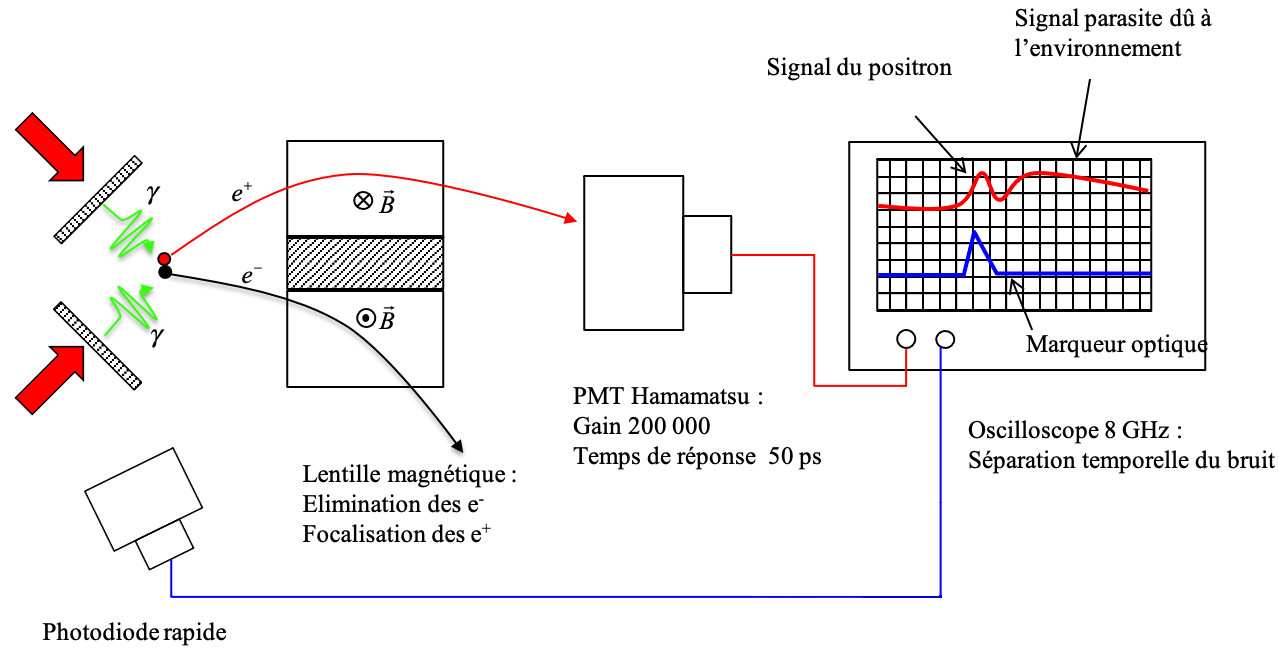
\includegraphics[width=\linewidth]{3-experience/chaine_comptage.png}
	\caption{Schéma de principe de la chaîne de comptage pour la détection du processus Breit-Wheeler linéaire dans un environnement bruité. Les flèches rouges représentent deux lasers, qui interagissant avec des cibles solides et produisent des photons $\gamma$ représentés en vert. Ces photons collisionnent et peuvent produire des paires électron-positron via le processus Breit-Wheeler linéaire. Les positrons sont focalisés sur une galette de micro-canaux par une lentille magnétique, pendant que électrons sont défocalisés. Le signal reçu est amplifié et envoyé sur un oscilloscope. L'arrivée du laser sur une des deux cibles permet de déterminer un temps initial et de séparer temporellement le signal voulu d'une partie importante du signal parasite produit par l'environnement proche du détecteur.}
	\label{fig:3-principe_comptage}
\end{figure}

Ainsi, ce dispositif permettrait de \textbf{compter les positrons un à un}, tout en \textbf{limitant le bruit de mesure} par un \textbf{filtrage temporel} (via le temps de réponse du détecteur et de l'oscilloscope), un \textbf{filtrage spatial} (via la géométrie de l'interaction, le blindage et la lentille magnétique) et un \textbf{filtrage énergétique} (via la lentille magnétique) dans une moindre mesure. De plus, le \textbf{décalage temporel progressif des deux lasers} permettrait aussi de pouvoir attribuer des positrons détectés au processus BWL spécifiquement. On s'attend en effet à ce que le \textbf{signal parasite} soit relativement \textbf{indépendant de la synchronisation des deux faisceaux de photons $\gamma$}, alors que le \textbf{signal de paires BWL} y sera \textbf{fortement dépendant}, puisque la production de paires par BWL aura lieu \textbf{uniquement si les photons $\gamma$ collisionnent entre eux}. 

Un prototype de la lentille a été réalisé par D. Khaghani durant son post-doctorat, et a été testée avec succès pour la focalisation d'électrons (courant inversé par rapport à la focalisation de positrons) sur le laser ECLIPSE 3, et avec un détecteur passif de type \textit{Imaging Plate}. Une application Geant4 permettant d'étudier le blindage est aussi en cours de développement par J.-L. Dubois. La démonstration expérimentale du fonctionnement de ce type de chaîne de comptage dans un environnement aussi bruité serait une première.

Cette configuration étant prévue pour le comptage \textbf{un à un} des positrons, il est néanmoins nécessaire d'\textbf{éviter les situations} où plusieurs particules pourraient être détectées en \textbf{coïncidence}, dans la même fenêtre temporelle.  Ce dispositif sera alors le plus efficace pour un nombre de positrons détecté typique de l'ordre de un positron tous les dix tirs. Comme ce schéma de comptage ne permet néanmoins pas de focaliser tous les positrons qui auraient pu être produits par le processus BWL sur le détecteur, nous nous fixerons dans le cadre de cette thèse un \textbf{objectif de production de paires} de l'ordre de \textbf{quelques positrons par tir laser}.


Dans le cadre de ce projet, un détecteur de photons $\gamma$ basé sur la diffusion Compton inverse linéaire d'électrons couplé à un spectromètre à électrons est aussi en cours développement par P. Forestier-Colleoni, en post-doctorat au LULI (Palaiseau). 

\newpage
\printbibliography[heading=subbibintoc]
\end{refsection}
